\documentclass[11pt]{article}

% ---------- Packages ----------
\usepackage[letterpaper,margin=1in]{geometry}
\usepackage[T1]{fontenc}
\usepackage{newtxtext,newtxmath}
\usepackage{microtype}
\usepackage{amsmath}  % newtxmath already provides the AMS symbols
\usepackage{booktabs,tabularx,array}
\usepackage{graphicx}
\usepackage[font=small,labelfont=bf]{caption}
\usepackage{float}
\usepackage{enumitem}
\usepackage{xcolor}
\usepackage{listings}
\usepackage[hidelinks]{hyperref}

\definecolor{codebg}{HTML}{F4F3EF}
\lstset{basicstyle=\ttfamily\footnotesize, backgroundcolor=\color{codebg},
        frame=none, xleftmargin=6pt, xrightmargin=6pt, aboveskip=6pt, belowskip=6pt,
        columns=fullflexible, keepspaces=true, breaklines=true}
\setlist{itemsep=2pt, topsep=4pt}
\graphicspath{{figures/}}
\newcolumntype{L}{>{\raggedright\arraybackslash}X}
\newcommand{\code}[1]{\texttt{#1}}
\newcommand{\E}{\mathbb{E}}

% ---------- Title ----------
\title{\textbf{Building the Raw Dataset for JPMorgan Chooser Option Pricing, 2018--2024}\\[4pt]
\large Week 1 Lab Report: Data Source Design and Initial Collection}
\author{Aiden Leong\\[2pt]
\small Goldman Sachs Online Internship, Quantitative Research \& Trading\\
\small Supervisor: Tyler Chan\\
\small \url{https://github.com/aiden-zl/advanced-chooser-option-pricing-model}}
\date{20 November 2026}

\begin{document}
\maketitle

\begin{abstract}
\noindent
I build the data layer for a re-implementation of the Black--Scholes--Merton (BSM) chooser option model of
Huang, Wang \& Wan~\cite{huang2021}. I configure and test connections to Yahoo Finance, FRED and Alpha Vantage against the live
services, and collect seven years (2018--2024) of JPMorgan Chase (JPM) daily prices and dividends, the VIX,
seven daily interest-rate series and two monthly macroeconomic series. All 23 automated data-quality
checks pass, including three cross-source checks in which Alpha Vantage matches Yahoo and FRED exactly. From the raw
data alone I recover the paper's spot price exactly (\$156.70) and its dividend yield to within 0.03 percentage
points; historical volatility comes out 1.0 point below the paper's 28.2\%, and the paper's 0.15\% risk-free rate
matches no Treasury yield on its valuation date. JPM's 21-day realized volatility ranges from 8.8\% to 135.3\%
over the sample, which is direct evidence against BSM's constant-volatility assumption and the motivation for the
machine-learning extensions planned in later weeks.
\end{abstract}

% =====================================================================
\section{Objective}
The project brief sets three tasks for Week~1:
\begin{enumerate}
  \item Write a data requirement specification covering financial, macroeconomic and sentiment data
        (delivered separately as \emph{Data Specification v1.0}).
  \item Configure and test the Yahoo Finance, Alpha Vantage and FRED APIs.
  \item Collect JPM daily prices, Treasury rates and the VIX for 2018--2024.
\end{enumerate}

% =====================================================================
\section{Background}
\subsection{The chooser option}
A (simple) chooser option gives its holder the right to decide at a \emph{choice date} $T_1$ whether the contract
becomes a European call or a European put, with common strike $K$ and common expiry $T_2 > T_1$~\cite{rubinstein1991}.
At $T_1$ a rational holder picks the more valuable of the two, so the payoff at the choice date is
\begin{equation}
  V_{T_1} \;=\; \max\!\bigl\{\, C(S_{T_1}, K, \tau),\; P(S_{T_1}, K, \tau) \,\bigr\}, \qquad \tau = T_2 - T_1,
  \label{eq:payoff}
\end{equation}
where $C$ and $P$ are the BSM call and put values with time $\tau$ remaining. Using put--call parity with a
continuous dividend yield $q$, the time-0 value decomposes into a call to $T_2$ plus a put to $T_1$~\cite{hull}:
\begin{equation}
  V_0 \;=\; C\bigl(S_0, K, T_2\bigr) \;+\; e^{-q\tau}\, P\!\bigl(S_0,\; K e^{-(r-q)\tau},\; T_1\bigr).
  \label{eq:decomp}
\end{equation}
Equation~\eqref{eq:decomp} is the closed-form benchmark for the Week~3 replication.

\subsection{The model to be replicated}
Huang et al.~\cite{huang2021} value a one-year JPM chooser by Monte-Carlo simulation of geometric Brownian motion.
The paper writes the drift as a generic $\alpha$; under risk-neutral pricing with a continuous dividend yield,
$\alpha = r - q$, which gives
\begin{equation}
  S_T \;=\; S_0 \exp\!\Bigl[\bigl(r - q - \tfrac12\sigma^2\bigr)T + \sigma\sqrt{T}\,Z\Bigr], \qquad Z\sim\mathcal N(0,1),
  \label{eq:gbm}
\end{equation}
with the fixed inputs in Table~\ref{tab:paper}. Every input except the contract terms ($K$, $T_1$, $T_2$) must
come from market data, which is what this week's dataset supplies.

\begin{table}[H]
\centering\small
\caption{Inputs used by Huang et al.~\cite{huang2021} (their Table~2), valuation date 23 August 2021.}
\label{tab:paper}
\begin{tabular}{@{}lrl@{}}
\toprule
Parameter & Value & Source in paper \\
\midrule
Spot price $S_0$         & \$156.70 & JPM close, 23 Aug 2021 \\
Volatility $\sigma$      & 28.2\%   & Historical, Aug 2020 -- Aug 2021 prices \\
Risk-free rate $r$       & 0.15\%   & Not stated \\
Dividend yield $q$       & 2.33\%   & Not stated \\
Strike $K$               & \$150    & CME option strike, 23 Aug 2021 \\
Choice date $T_1$        & 0.5 y    & Contract term \\
Expiry $T_2$             & 1 y      & Contract term \\
\bottomrule
\end{tabular}
\end{table}

% =====================================================================
\section{Methods}
\subsection{Environment and security}
Python~3.14 in a virtual environment with pandas~3.1, NumPy~2.5, yfinance~1.8, fredapi~0.5, requests~2.34
and Matplotlib~3.11. API keys are held in a git-ignored \code{.env} file, since the repository is public.

\subsection{Connection scripts}
Each data source has its own module with a live connection test (Table~\ref{tab:modules}); a single command,
\code{python -m src.pull\_all}, runs all three tests, downloads every dataset, runs the validation suite and writes
a dated manifest.

\begin{table}[H]
\centering\small
\caption{Connection modules and what each live test verifies.}
\label{tab:modules}
\begin{tabularx}{\linewidth}{@{}>{\ttfamily}p{0.36\linewidth}L@{}}
\toprule
\normalfont Module & Live connection test \\
\midrule
src/data\_sources/yahoo.py & Downloads JPM for 20--24 Aug 2021 and asserts the 23 Aug close equals the paper's \$156.70. \\
src/data\_sources/fred.py & Downloads the 1-year Treasury yield (\code{DGS1}) around the same date. \\
src/data\_sources/alpha\_vantage.py & One uncached \code{GLOBAL\_QUOTE} call. Detects Alpha Vantage's ``HTTP 200 with an error message'' responses, rate-limits to one call per 1.5\,s and caches responses to protect the daily quota. \\
src/pull\_all.py & Runs the three tests, the full pull and the 23-check validation suite; writes \code{data/raw/manifest.json}. \\
\bottomrule
\end{tabularx}
\end{table}

\subsection{Design decisions}
\begin{itemize}
  \item \textbf{Unadjusted and adjusted prices.} Data are pulled with \code{auto\_adjust=False}. The paper's $S_0$ is
        the unadjusted close; the dividend-adjusted close is about \$19 lower on the same day and would misstate $S_0$.
  \item \textbf{Inclusive end date.} \code{yfinance} treats its end date as exclusive, so one day is added to keep
        31 December 2024.
  \item \textbf{No cleaning at this stage.} Holiday blanks in the FRED series are kept as received; interpolation and
        outlier handling are Week~2 tasks, so every transformation stays traceable.
  \item \textbf{Alpha Vantage as a cross-check.} On the free key, full daily price history and news sentiment are
        premium features (confirmed by the API's own responses). Yahoo is therefore the primary price source and Alpha
        Vantage independently verifies dividends, month-end prices and Treasury yields.
\end{itemize}

\subsection{Estimators}
Daily log returns are $r_t = \ln(S_t/S_{t-1})$. Annualized historical volatility over a window of $n$ returns is
\begin{equation}
  \hat\sigma \;=\; \sqrt{252}\,\sqrt{\frac{1}{n-1}\sum_{t=1}^{n}\bigl(r_t-\bar r\bigr)^2},
  \label{eq:vol}
\end{equation}
and the trailing dividend yield on date $t$ is $\hat q_t = \bigl(\sum_{i\,:\,t-1\text{y} < t_i \le t} D_i\bigr)/S_t$,
the sum of cash dividends with ex-dates in the preceding year divided by the spot price. Rolling versions of
\eqref{eq:vol} with $n=21$ and $n=252$ are used in Figure~\ref{fig:vol}.

% =====================================================================
\section{Results}
\subsection{Connection tests}
All three services responded correctly on 20 November 2026:
\begin{lstlisting}
[yahoo] OK  JPM close on 2021-08-23 = 156.70 (paper: 156.7)
[fred]  OK  DGS1 on 2021-08-23 = 0.07%  (10 obs)
[alpha] OK  JPM latest trading day 2026-11-20, price 310.53
\end{lstlisting}

\subsection{Raw dataset}
\begin{table}[H]
\centering\small
\caption{Files in \code{data/raw/} (2018-01-01 to 2024-12-31).}
\label{tab:files}
\begin{tabularx}{\linewidth}{@{}>{\ttfamily}p{0.36\linewidth}Lr@{}}
\toprule
\normalfont File & Content & Rows \\
\midrule
yahoo\_jpm\_daily.csv & JPM open, high, low, close, adjusted close, volume, dividends, splits & 1,761 \\
yahoo\_vix\_daily.csv & VIX daily bars & 1,761 \\
fred\_daily.csv & DTB3, DGS3MO, DGS6MO, DGS1, DGS2, DGS10, DFF, VIXCLS & 2,557 \\
fred\_monthly.csv & CPIAUCSL, UNRATE & 84 \\
av\_jpm\_dividends.csv & Dividend history (cross-check) & 28 \\
av\_jpm\_monthly\_adjusted.csv & Month-end prices (cross-check) & 84 \\
av\_treasury\_\{3month,10year\}.csv & Daily Treasury yields (second source) & 1,827 each \\
av\_jpm\_daily\_compact.csv & Most recent 100 trading days (free-tier cap) & 100 \\
\bottomrule
\end{tabularx}
\end{table}

\subsection{Data-quality validation}
All 23 checks pass. They cover row counts and date coverage, a shared JPM/VIX trading calendar, the paper anchor
price, price ranges, dividends in both sources, Alpha Vantage against Yahoo and FRED, Yahoo against FRED for the VIX,
and the completeness of every FRED series. Eight checks failed on the first run; in each case the data were correct
and the check was mis-specified. FRED's fed funds series (\code{DFF}) is published every calendar day, which adds
weekend rows to the combined table, and the VIX tolerance was tighter than the two sources' real differences.
The checks now judge each series on weekdays only and require VIX agreement on at least 99.5\% of days. After the
fix, the Treasury series are blank on 77 of 1,827 weekdays (4.2\%, bond-market holidays) and the two VIX sources agree
to within 0.01 on 1,759 of 1,761 days. The Alpha Vantage cross-checks match exactly: all 28 dividends (dates and
amounts), all 84 month-end closes, and the 3-month and 10-year yields on all 1,750 days shared with FRED.

\subsection{Re-deriving the paper's inputs}
\begin{table}[H]
\centering\small
\caption{Paper inputs versus values computed from the raw data on 23 August 2021.}
\label{tab:rederive}
\begin{tabular}{@{}lrrl@{}}
\toprule
Input & Paper & My data & Status \\
\midrule
$S_0$: JPM unadjusted close                         & \$156.70 & \$156.70 & Exact \\
$q$: trailing 12-month dividends / $S_0$             & 2.33\%   & 2.30\%   & Within 0.03 pt \\
$\sigma$: eq.~\eqref{eq:vol}, 252 returns to 23 Aug 2021 & 28.2\%   & 27.2\%   & 1.0 pt lower \\
$r$: 1-year Treasury (\code{DGS1})                  & 0.15\%   & 0.07\%   & No tenor matches \\
\bottomrule
\end{tabular}
\end{table}

To explain the $\sigma$ gap I recomputed volatility under 272 conventions: log or simple returns, adjusted or
unadjusted prices, sample or population standard deviation, annualization by 250, 252 or 365 days, eleven window
start dates, and weekly or monthly sampling. The closest result is 27.7\% and none gives 28.2\%. Because $S_0$
matches to the cent, the price data are not the cause; the gap most likely comes from a calculation step the paper
does not describe. For $r$, every Treasury yield on that date (0.05\% to 0.23\%) differs from 0.15\%. One hypothesis
is 6-month USD LIBOR, whose tenor matches $T_1$; it is unverified because FRED no longer hosts LIBOR. Week~3 will
price the option with both the paper's inputs and my data-derived inputs to measure how much these gaps matter.

\subsection{Exploratory analysis}

\begin{figure}[H]
\centering
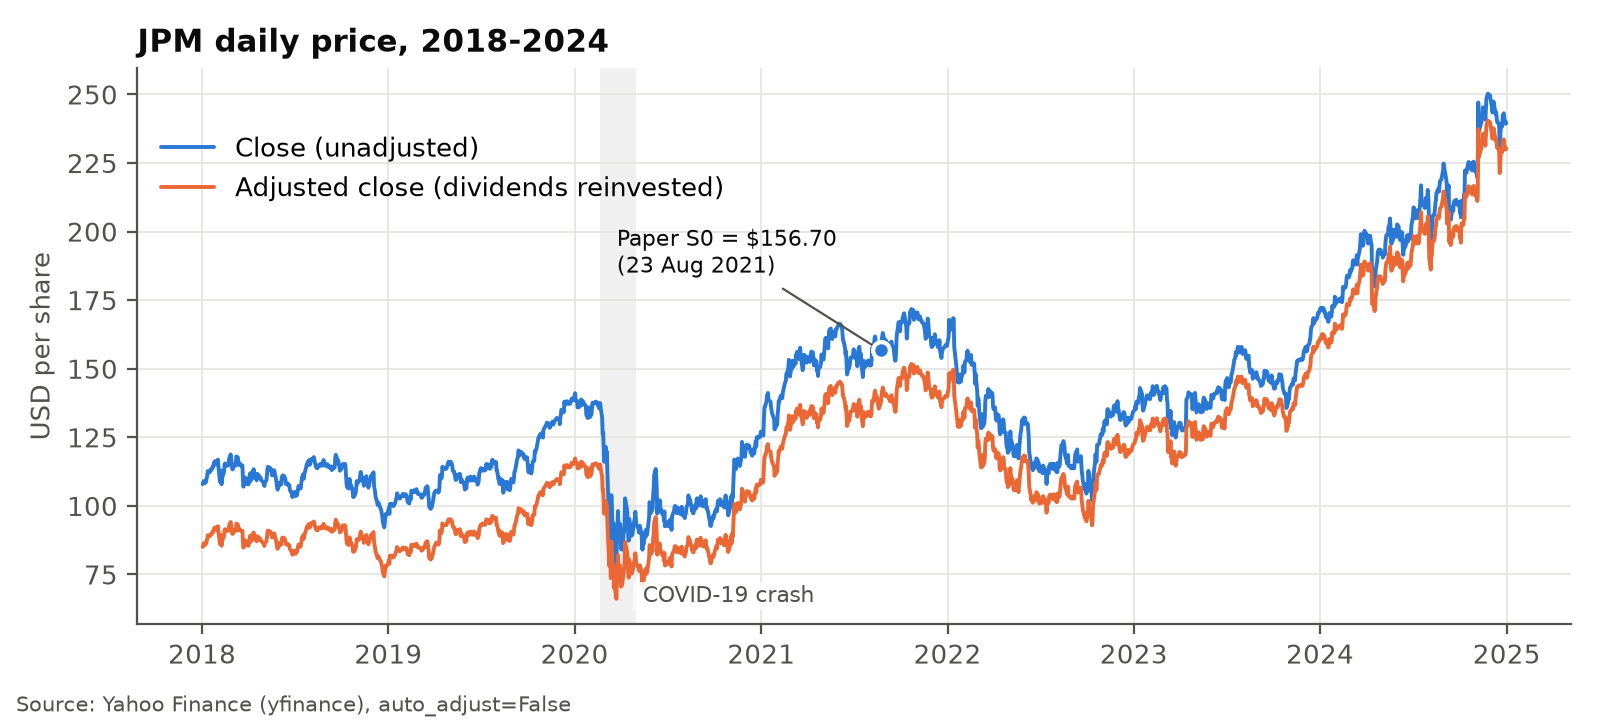
\includegraphics[width=\linewidth]{fig1_jpm_price.png}
\caption{JPM daily close, 2018--2024. The unadjusted close rose from \$107.95 to \$239.71, with a low of \$79.03
on 23 March 2020 (COVID-19 crash) and a high of \$250.29 on 25 November 2024. The marker shows the paper's valuation
date and $S_0$.}
\label{fig:price}
\end{figure}

\begin{figure}[H]
\centering
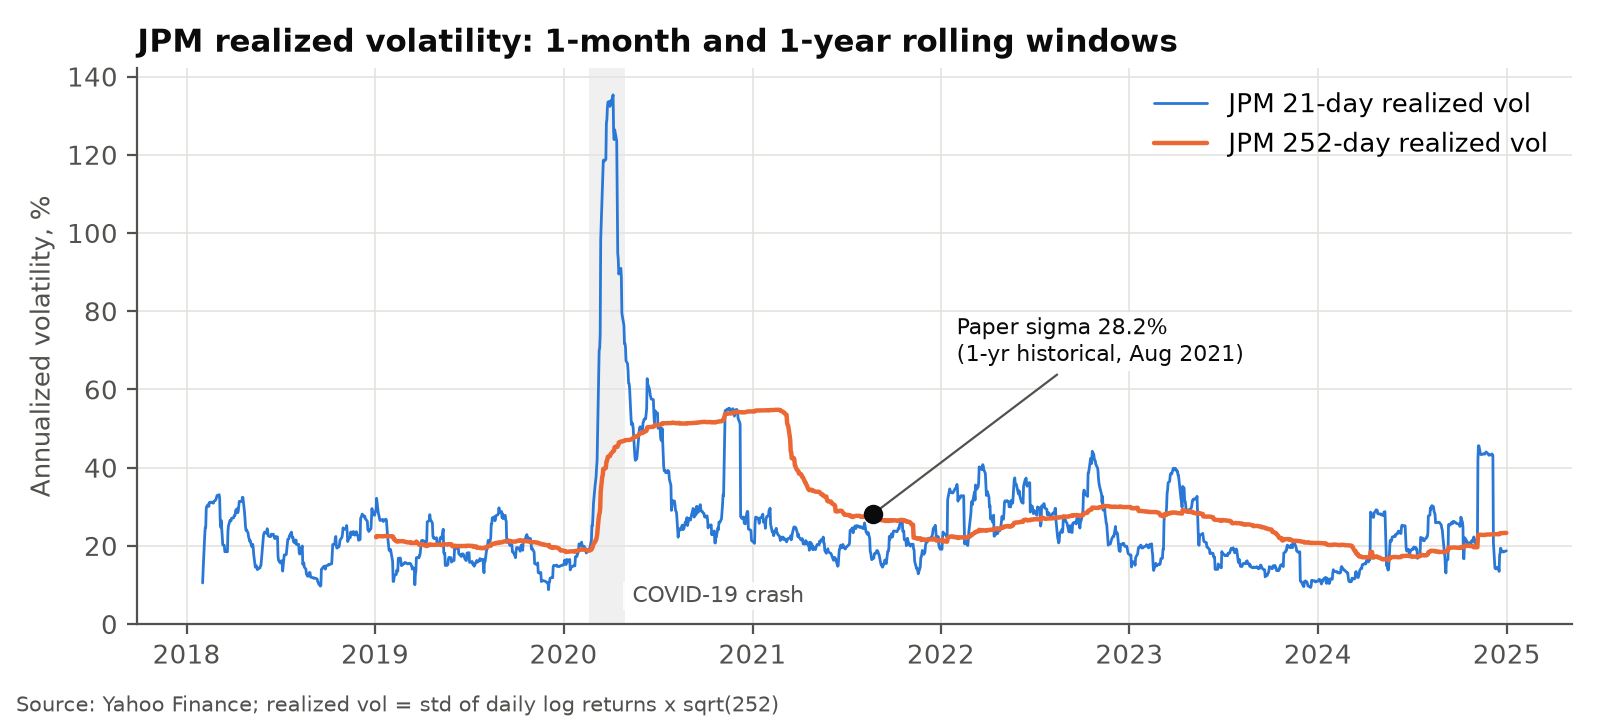
\includegraphics[width=\linewidth]{fig4_volatility.png}
\caption{Volatility is not constant. JPM's 21-day realized volatility ranges from 8.8\% to 135.3\%, and annual
realized volatility was 54.3\% in 2020 against 18.8\%--30.0\% in other years. Each point is the volatility over the
window ending on that date; the dot is the paper's $\sigma = 28.2\%$. A single $\sigma$ cannot capture these regimes.}
\label{fig:vol}
\end{figure}

\begin{figure}[H]
\centering
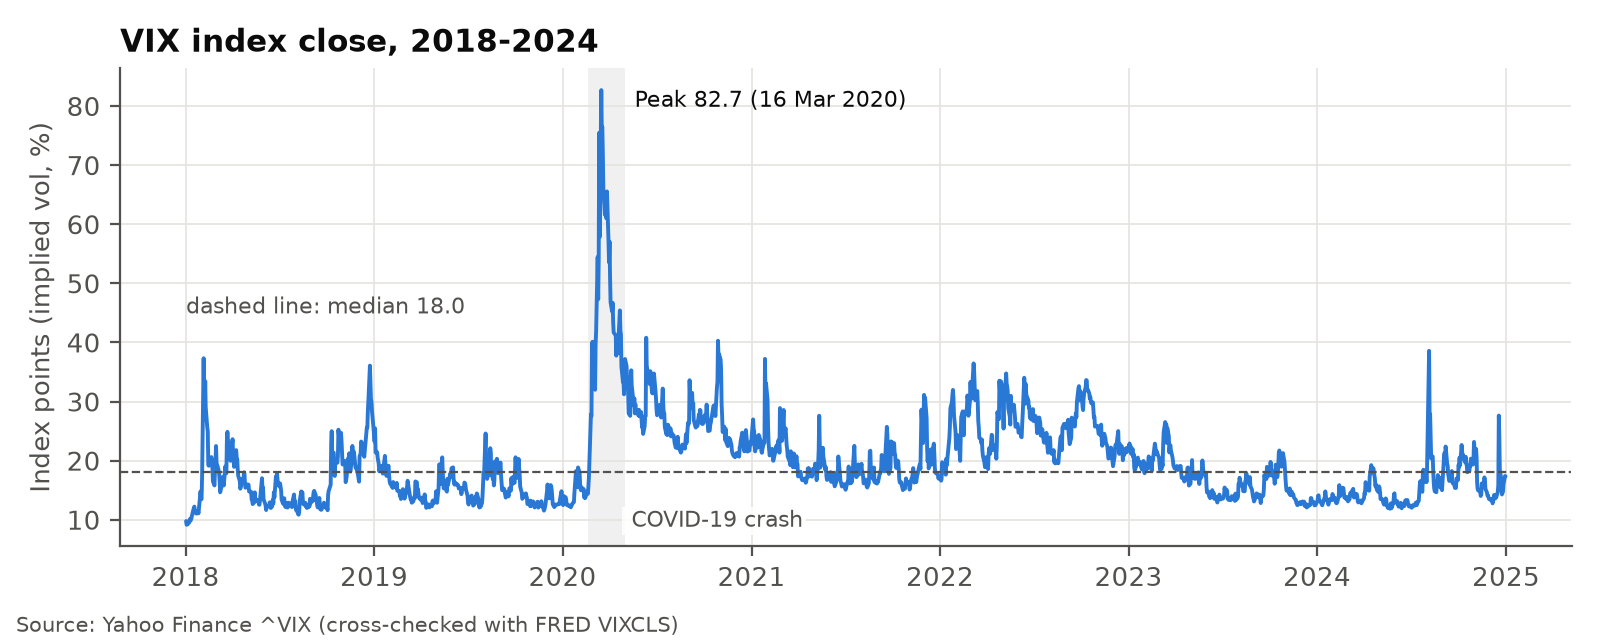
\includegraphics[width=\linewidth]{fig2_vix.png}
\caption{VIX daily close from Yahoo Finance. Data check: values stay in a plausible range (9.15 to 82.69), there
are no gaps, and the March 2020 spike appears where expected. Yahoo matches FRED's \code{VIXCLS} on 1,759 of 1,761 days.}
\label{fig:vix}
\end{figure}

\begin{figure}[H]
\centering
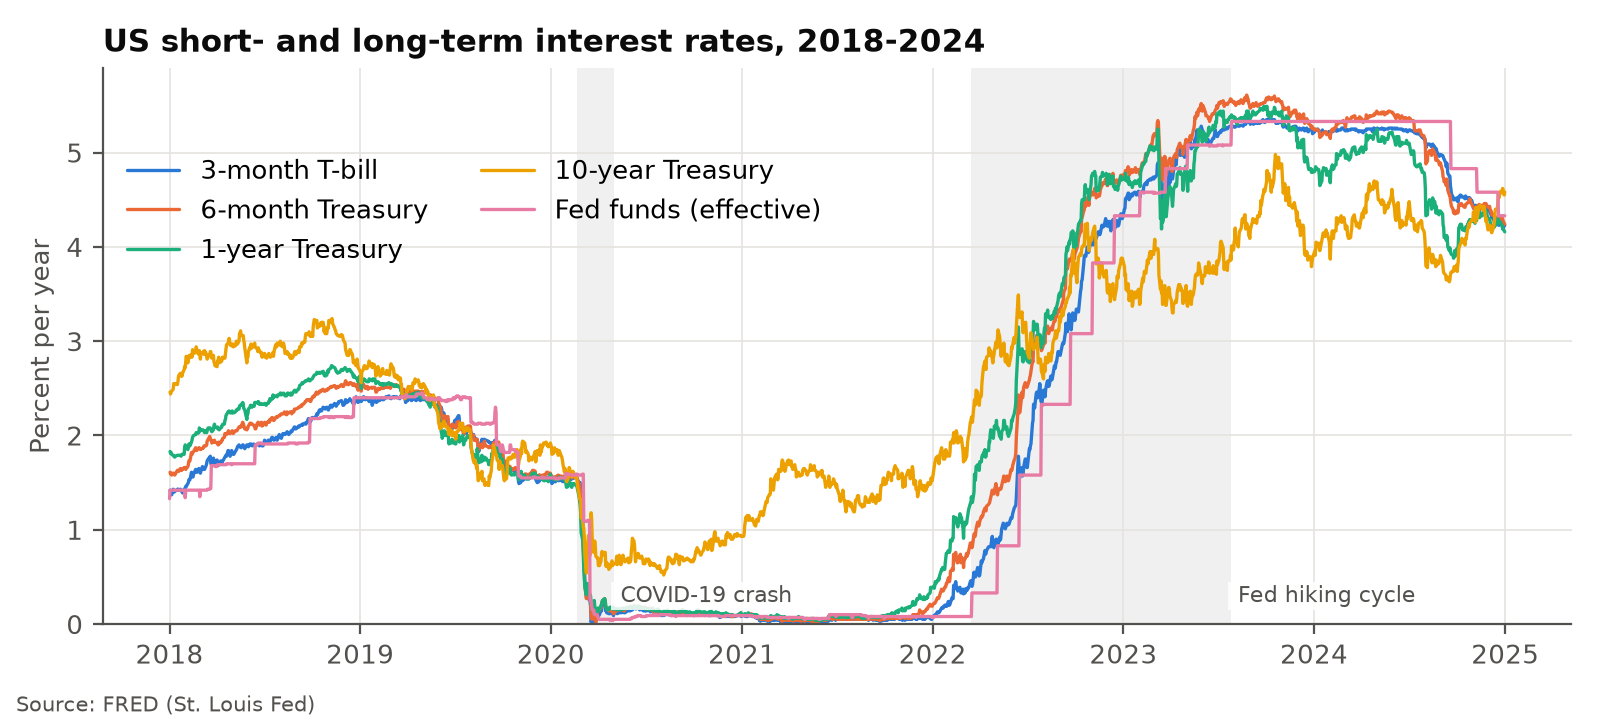
\includegraphics[width=\linewidth]{fig3_rates.png}
\caption{Interest-rate series from FRED. Data check: all five series are in percent per year, have no gaps beyond
bond-market holidays, and show the known rate cuts in March 2020 and rate hikes from 2022.}
\label{fig:rates}
\end{figure}

\begin{figure}[H]
\centering
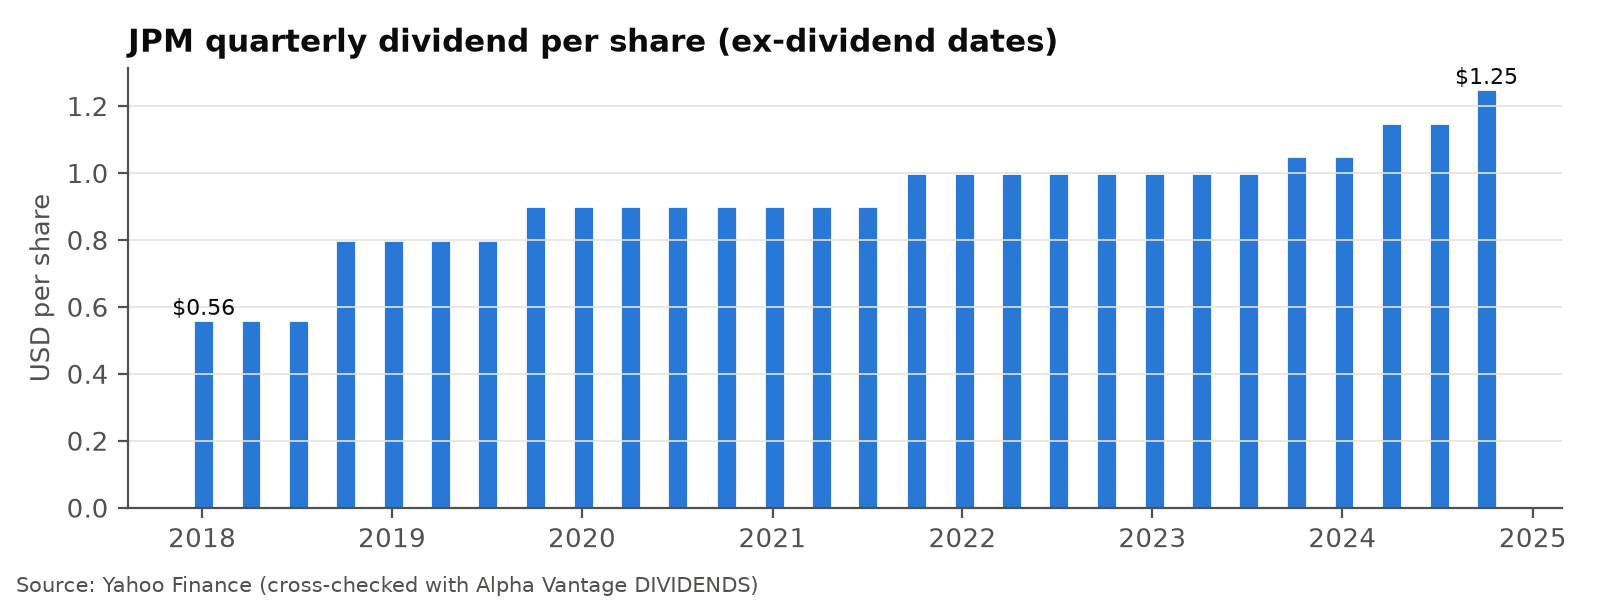
\includegraphics[width=\linewidth]{fig5_dividends.png}
\caption{JPM quarterly dividends per share from Yahoo Finance. Data check: 28 payments, one per quarter, with no
missing quarters; Alpha Vantage reports the same 28 ex-dates and amounts.}
\label{fig:div}
\end{figure}

% =====================================================================
\section{Discussion}
\paragraph{The data support the project's premise.} Volatility (Figure~\ref{fig:vol}) and rates
(Figure~\ref{fig:rates}) both change regime several times within the sample, so a model with constant $\sigma$ and
$r$ will misprice systematically across regimes. That is the gap the machine-learning weeks target.

\paragraph{Limitations of the sources.} Yahoo is an unofficial free source and can revise its history. I mitigate
this by cross-checking against FRED and Alpha Vantage and by committing the raw files with a dated manifest. Alpha
Vantage's free tier cannot supply full daily history or news sentiment.

\paragraph{Risks for later weeks.} (i) Historical option prices for the Week~4 error metrics: JPM single-stock
options trade on US equity options exchanges rather than CME, and 2018--2024 history is a commercial product.
(ii) Historical sentiment: NewsAPI's free tier covers only about the last 30 days. The data specification lists
alternatives and the decisions required.

% =====================================================================
\section{Conclusion and next steps}
All three Week~1 deliverables are complete: the data specification, working connection scripts for three APIs, and
a validated 2018--2024 raw dataset. Week~2 will clean and align the data (interpolation, IQR outlier screening,
alignment to the NYSE calendar) and construct at least ten features, including rolling volatilities, returns,
dividend growth, the VIX--JPM correlation, interest-rate momentum and sentiment, with GitHub Actions scheduling the
pipeline.

% =====================================================================
\appendix
\section{Reproducing these results}
\begin{lstlisting}
git clone https://github.com/aiden-zl/advanced-chooser-option-pricing-model
cd advanced-chooser-option-pricing-model
python3 -m venv .venv && source .venv/bin/activate
pip install -r requirements.txt
cp .env.example .env          # add your FRED and Alpha Vantage keys
python -m src.pull_all        # connection tests, raw pull, 23 validation checks
python -m src.week1_figures   # figures and deliverables/week1/week1_stats.json
tectonic deliverables/week1/lab_report.tex   # rebuild this PDF
\end{lstlisting}

% =====================================================================
\begin{thebibliography}{9}\small
\bibitem{huang2021} Z.~Huang, X.~Wang and W.~Wan. Exploration of JPMorgan chooser option pricing.
  \emph{BCP Business \& Management}, 15:93--102, 2021.
\bibitem{rubinstein1991} M.~Rubinstein. Chooser options. 1991. (As cited in the project brief.)
\bibitem{hull} J.~C.~Hull. \emph{Options, Futures, and Other Derivatives}. Pearson. Chapter on exotic options.
\end{thebibliography}

\end{document}
